% Written by src/detection/final_figures.py; needs \usepackage{graphicx} and results/figures/ in \graphicspath.
\begin{figure}[tb]
  \centering
  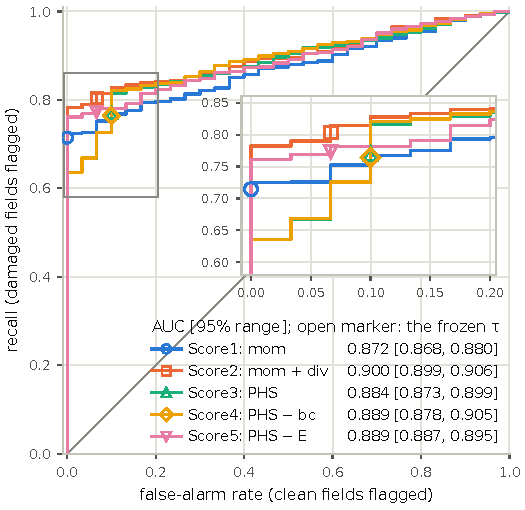
\includegraphics[width=\columnwidth]{fig_roc.pdf}
  \caption{ROC curves of the five scores on the 930 fields of the 30 new cases (900 damaged, 30 clean); the inset enlarges the top-left corner. Legend: AUC [95\% confidence interval: case bootstrap, 2000 resamples of whole cases within each $k$]. Markers: the frozen $\tau$ of each score, at its false-alarm rate on the 30 clean fields and its recall (Score3 and Score4 nearly coincide: 3 false alarms each, 693 and 688 damaged fields flagged); the false-alarm axis moves in steps of 1/30. The intervals lean above their estimates (Score2: 0.900 [0.899, 0.906]), and for 3 subsets in Tables~\ref{tab:benchmark_metrics_by_k} and \ref{tab:benchmark_metrics_by_type} they lie entirely above them, e.g. Score4 for $k = 1$ (Table~\ref{tab:benchmark_metrics_by_k}): 0.927 [0.928, 0.941]. A resample that draws a case twice adds the pairs of that case's clean field with its own damaged fields, which are nearly always in the right order (there, 98.3\% of them, against 92.0\% of the pairs across cases), so the resampled AUCs run high. Score terms: mom, the momentum residual; div, the continuity residual; bc, the boundary-localization term; E, the energy-decay term; PHS, the sum of all four, each divided by its mean over the calibration fields.}
  \label{fig:roc}
\end{figure}
